% Agentic Fraud Detection System Paper
% Based on Springer LNCS template

\documentclass{svproc}

\usepackage{url}
\usepackage{helvet}
\usepackage{courier}
\usepackage{color}
\usepackage{makeidx}
\usepackage{graphicx}
\usepackage[misc]{ifsym}
\usepackage{multicol}
\usepackage[bottom]{footmisc}
\usepackage{tabularx}
\usepackage{longtable}
\usepackage{rotating}
\usepackage{amsmath}
\usepackage{subfig}
\usepackage{algorithm}
\usepackage{algorithmic}

\def\UrlFont{\rmfamily}

\begin{document}
\mainmatter

\title{Agentic Fraud Detection System using MAPE-K Architecture}

\titlerunning{Agentic Fraud Detection using MAPE-K}  

\author{Priti Gupta\inst{1}}

\authorrunning{P. Gupta}

\institute{Your Institution, City, Country \\
\email{youremail@institution.com}}

\maketitle

\begin{abstract}
Fraud detection systems face significant challenges including class imbalance, concept drift, and adversarial evasion attacks. This paper presents an automated fraud detection system built on the MAPE-K (Monitor-Analyze-Plan-Execute using Knowledge) architecture that autonomously adapts to evolving fraud patterns. The system integrates: social media-based data collection and LLM-driven annotation, CTGAN-based data augmentation, adversarial training for robustness, and a closed-loop MAPE-K framework with five specialized agents following the M $\rightarrow$ A $\rightarrow$ Decision $\rightarrow$ P $\rightarrow$ E order with active Knowledge Base. Our system achieves F1 of 0.9911, ROC-AUC of 0.9966, and 98.34\% robustness. The MAPE-K loop detects drift via PSI/KS, triggers automatic retraining when needed, and includes a Supervisor with convergence monitoring.

\keywords{Fraud Detection, MAPE-K Architecture, Adversarial Training, Data Drift, CTGAN, Autonomous Systems}
\end{abstract}

\section{Introduction}\label{sec:intro}
Fraud is a major issue in today's digital economy. Financial losses from fraudulent transactions reach billions of dollars annually, affecting both businesses and individuals. Many fraud detection systems exist, but they face three key challenges. First, most datasets have far more normal transactions than fraudulent ones, making it hard for models to learn what fraud looks like \cite{dalpozzolo2015credit}. Second, fraud patterns change over time as scammers develop new techniques - this is called concept drift \cite{card2017}. Third, fraudsters can deliberately manipulate their behavior to bypass detection systems.

Most existing approaches use single machine learning models that cannot adapt when patterns change. Some systems use rule-based methods, but these struggle to keep up with evolving fraud. Other solutions exist for individual problems like class imbalance or adversarial attacks, but fewer systems handle all three challenges together.

This paper aims to build an automated fraud detection system that can adapt automatically. We use the MAPE-K architecture, where automated modules monitor the system, analyze conditions, plan responses, and execute actions. This allows the system to detect when fraud patterns shift and retrain itself without human help.

We gathered data from social media platforms where people share their scam experiences. Large language models help label this data automatically. To handle class imbalance, we use CTGAN to create more examples of normal transactions. We also train the model with adversarial examples so it stays robust even when attacked. The MAPE-K agents tie everything together, checking for drift and deciding when to retrain.

The main contributions of this work are a complete automated fraud detection pipeline that collects data, augments it, trains robustly, and adapts on its own, implementation of MAPE-K architecture for fraud detection that can measure how well the model learns over time, demonstration that combining CTGAN with adversarial training achieves 98.34\% robustness, and demonstrates promising experimental results F1 score of 0.9911 and ROC-AUC of 0.9966.

\section{Related Work}\label{sec:related}
Fraud detection has been widely studied in the literature. Traditional approaches use rule-based systems and basic machine learning models like logistic regression and decision trees. More recent work applies deep learning methods to detect fraudulent transactions. However, these approaches typically treat fraud detection as a static classification problem and do not address the challenges of changing fraud patterns.

Class imbalance is a well-known challenge in fraud detection. Dal Pozzolo et al. \cite{dalpozzolo2015credit} studied credit card fraud detection and showed that class imbalance significantly affects model performance. Various techniques have been proposed to handle this, including undersampling, oversampling, and synthetic data generation. CTGAN, introduced by Xu et al. \cite{xu2019ctgan}, generates synthetic tabular data that preserves the statistical properties of the original dataset. Several works have applied CTGAN to fraud detection with promising results \cite{strelcenia2023synthetic}.

Concept drift is another critical issue in fraud detection. As fraudsters change their tactics, the data distribution shifts over time. Goudar et al. \cite{goudar2026adaptive} proposed adaptive bagging strategies to address concept drift in fraud detection systems. Various drift detection methods exist, including population stability index and Kolmogorov-Smirnov tests.

Adversarial robustness has gained attention in recent years. Madry et al. \cite{madry2018adversarial} showed that adversarial training can improve model robustness against evasion attacks. For tabular data, Simonetto et al. \cite{simonetto2024tabularbench} introduced TabularBench to benchmark adversarial robustness. Melo et al. \cite{melo2023adversarial} explored adversarial training specifically for tabular fraud detection data.

The MAPE-K architecture, introduced by IBM \cite{ibm2005autonomic}, provides a framework for building self-managing systems. Recent work has applied MAPE-K to various domains including microservices \cite{bucchiarone2022mape} and cloud systems \cite{oh2023mape}. However, limited work has explored MAPE-K for fraud detection specifically.

Our work differs from existing approaches by building an automated system that integrates data collection, augmentation, adversarial training, and autonomous adaptation using the MAPE-K architecture.

\section{Methodology}\label{sec:methodology}
This section describes the four main components of our automated fraud detection system.

\subsection{Data Collection and Annotation}
We collected fraud-related data from social media platforms where people share their scam experiences. The data collection process involved two main steps.

First, we scraped posts from Reddit fraud-focused communities (e.g., r/Scams, r/antiScam, r/fraud) along with their comments, using targeted keywords related to common fraud types such as investment scams, phishing, and payment fraud. The scraping targeted posts from the past several months to capture recent fraud patterns. We collected post content, comments, timestamps, and user interactions.

Second, we used the Llama3 Instruct model to automatically label the collected data. The LLM was prompted as an expert fraud analyst to identify whether each post described actual fraud using the post and its comments, extract the type of fraud if present, note the currency involved, extract the amount mentioned, and identify psychological tactics used (e.g., urgency, fear, authority). The LLM provided three labels: fraud (1), non-fraud (0), and uncertain (-1), along with confidence scores. Posts with confidence scores below 0.7 or labeled as uncertain (-1) were filtered out to ensure data quality. This two-stage filtering (uncertain labels and low-confidence) ensures high-quality labeled examples for training.

To validate the Llama3 annotation quality, we conducted a multi-stage validation. First, 200+ samples were verified using GPT-5 to cross-check Llama3 annotations. Second, 100+ samples were manually verified by the authors. This confirms the reliability of the Llama3-based annotation approach.

\subsection{Data Augmentation using CTGAN}
Many fraud detection datasets have class imbalance, with fraud as the minority class. However, our Reddit-sourced dataset has the opposite distribution: approximately 95\% fraud and 5\% non-fraud, because we specifically scraped from fraud-focused communities where users share their scam experiences. This makes non-fraud the minority class at only 5\%. We use CTGAN, a generative adversarial network designed for tabular data \cite{xu2019ctgan}, to generate synthetic non-fraud examples to balance the dataset.

CTGAN consists of two neural networks that work against each other. The generator creates synthetic data that looks real, while the discriminator tries to distinguish between real and fake data. Through training, the generator learns to produce realistic samples that match the statistical properties of the original data.

We trained CTGAN on our minority class examples, which in this case are the normal transactions. The trained model generates new synthetic examples of normal transactions. These synthetic examples help balance the dataset, giving the model more examples to learn from.

To ensure the quality of synthetic data, we validated it using statistical tests. We compared the distribution of synthetic data with real data using Jensen-Shannon Divergence to ensure the generated samples maintain the same statistical properties as the original dataset.

\subsection{Adversarial Training}
Fraudsters can deliberately try to trick detection systems by modifying their transaction patterns. To make our model robust against such attacks, we employ adversarial training using the Fast Gradient Sign Method (FGSM) \cite{madry2018adversarial}.

Given an input feature vector $\mathbf{x}$ with label $y$, the adversarial example is generated as:

\begin{equation}
\mathbf{x}_{adv} = \mathbf{x} + \epsilon \cdot \text{sign}(\nabla_{\mathbf{x}} \mathcal{L}(\theta, \mathbf{x}, y))
\end{equation}

where $\epsilon = 0.05$ is the perturbation magnitude (5\% of feature range), $\nabla_{\mathbf{x}} \mathcal{L}$ is the gradient of the loss function with respect to the input features, and $\theta$ represents the model parameters. The sign operation ensures perturbations are in the direction that maximizes the loss.

During training, the model is exposed to both clean examples $(\mathbf{x}, y)$ and adversarial examples $(\mathbf{x}_{adv}, y)$. This enables the model to learn robust decision boundaries that remain effective even when input features are maliciously perturbed. The model is trained to correctly classify both clean and adversarial examples, improving robustness against evasion attacks without significantly degrading performance on clean data \cite{goodfellow2014gan}.

We evaluate robustness by measuring performance degradation under different perturbation strengths $\epsilon \in \{0.01, 0.05, 0.10, 0.20, 0.30\}$. The robustness score is calculated as the ratio of F1 score under attack to clean F1 score.

\subsection{Autonomous Adaptation Layer: MAPE-K Architecture}

The autonomous adaptation layer implements the MAPE-K (Monitor--Analyze--Plan--Execute over a shared Knowledge base) paradigm to enable continuous self-regulation of the system. Unlike static machine learning pipelines, the proposed framework operates as a closed-loop control system that autonomously monitors system behavior, evaluates model performance, and triggers corrective actions based on predefined policies and historical knowledge.

While the system does not employ policy learning or reasoning-based agents, it achieves autonomy through structured feedback loops and rule-based decision mechanisms, consistent with autonomic computing principles.

The system operates in two distinct phases:

\begin{enumerate}
    \item \textbf{Training Phase (One-time):} The initial pipeline executes once to prepare the model for deployment. This phase consists of: Ingestion (data collection from social media), Annotation (LLM-based labeling), Augmentation (CTGAN to balance classes), Training (adversarial training for robustness), and Initial Deployment.
    
    \item \textbf{Monitoring Phase (Continuous):} After deployment, the MAPE-K control loop runs continuously to enable autonomous. This phase monitors live data, detects drift or performance degradation, and automatically triggers retraining when needed. This is where the autonomous capability resides.
\end{enumerate}

The proposed adaptation layer adopts the MAPE-K paradigm. The architecture follows the canonical MAPE-K control loop, with each phase implemented as a specialized functional module:

\begin{itemize}
    \item \textbf{Monitoring (M) -- Drift Detection}: Continuously detects concept drift in incoming data using statistical measures such as Population Stability Index (PSI) and Kolmogorov--Smirnov (KS) tests. These are evaluated against historical distributions stored in the Knowledge Base.

    \item \textbf{Analysis (A) -- Performance Evaluation}: Evaluates model performance using metrics including F1-score, ROC-AUC, and robustness. The agent compares current performance with baseline metrics retrieved from the Knowledge Base to determine if adaptation is needed.

    \item \textbf{Decision Engine}: Determines the system's operational path using threshold-based control policies that incorporate both real-time metrics and historical information from the Knowledge Base. If performance meets predefined thresholds and no drift is detected, the model continues in production. Otherwise, corrective adaptation is triggered through the planning phase.

    \item \textbf{Planning (P) -- Training Strategy}: Defines an appropriate adaptation strategy, which may involve model retraining, hyperparameter adjustment, or data recollection. The planning phase leverages historical configurations and prior outcomes stored in the Knowledge Base to guide decision-making and enable the system to learn from past adaptations.

    \item \textbf{Execution (E) -- Retraining and Deployment}: Executes the planned strategy, including data augmentation using CTGAN and adversarial training. The updated model is then prepared for deployment, and the cycle repeats.
\end{itemize}

The critical distinction is that the MAPE-K loop operates \textbf{continuously after deployment}, not during initial training. Each adaptation cycle enables the system to learn from previous experiences, making it a genuine autonomous system.

The Knowledge Base serves as a centralized historical repository that supports all phases of the MAPE-K loop. It stores historical drift statistics (PSI/KS values over time) for drift comparison in the Monitoring phase, baseline and past performance metrics for evaluation in the Analysis phase, training configurations including hyperparameters and augmentation strategies for reuse during Planning, and deployment history and model versions to support informed decision-making. Each component both retrieves from and updates the Knowledge Base, enabling cumulative learning and improved adaptation over time. This is the key to autonomous: the system remembers what worked and what didn't, and uses this knowledge to make better decisions in future adaptation cycles.

The system incorporates multiple feedback mechanisms to enable adaptive behavior at different levels:

\begin{itemize}
    \item \textbf{L1 (Data-level Adaptation)}: Decision $\rightarrow$ Execution. Data is rebalanced using CTGAN when performance degradation is detected.

    \item \textbf{L2 (Model-level Adaptation)}: Decision $\rightarrow$ Planning. Training strategies are modified (e.g., hyperparameters, adversarial strength) when performance falls below threshold.

    \item \textbf{L3 (Re-evaluation Loop)}: Planning $\rightarrow$ Monitoring. Drift and performance are re-evaluated after retraining to validate improvement.

    \item \textbf{L4 (Supervisory Control)}: A supervisory mechanism enforces operational constraints, including a maximum of three adaptation iterations, early convergence detection ($\Delta F1 < 0.01$), and instability handling (e.g., aborting when $F1 < 0.5$ after multiple iterations).

    \item \textbf{L5 (Knowledge Update)}: Decision $\rightarrow$ Knowledge Base. System states, performance metrics, drift observations, and configurations are persistently stored for future reference.
\end{itemize}

During the monitoring phase, the system operates as an iterative closed-loop autonomous process: Monitoring continuously detects concept drift by comparing incoming data distributions with historical baselines; Analysis evaluates model performance using predefined metrics and thresholds; Decision determines whether to retain the current model or initiate adaptation; Planning formulates an adaptation strategy based on what worked in previous cycles; Execution applies data augmentation and adversarial training, followed by model update and deployment; Iteration repeats the cycle enabling the system to continuously learn and improve.

The system thus achieves autonomous capability by detecting degradation triggers (drift or poor performance), planning appropriate responses based on historical knowledge (data or model-level corrections), executing changes, and verifying outcomes---all while leveraging the Knowledge Base to improve future decisions through accumulated experience.

\begin{figure}
\centering

\includegraphics[width=0.8\textwidth]{architecture.png}
\caption{System Architecture: MAPE-K based Agentic Fraud Detection System}
\label{fig:architecture}
\end{figure}

\section{Experimental Setup}\label{sec:experimental}
This section describes our experimental setup including the dataset, model configuration, and evaluation metrics.

\subsection{Dataset}
We used a dataset collected from social media platforms containing labeled fraud examples. The dataset consists of posts labeled as either fraudulent or normal (non-fraud). The data was collected over a period of several months from Reddit fraud-focused communities.

The raw dataset contained 9,000 posts scraped from Reddit fraud forums. The LLM annotation provided three labels: fraud (1), non-fraud (0), and uncertain (-1). After removing approximately 4,000 posts labeled as uncertain, we retained 5,000 labeled examples. For experimentation, we used a subset of 3,000 examples.

Unlike typical fraud datasets where fraud is the minority class (e.g., credit card fraud), our dataset contains more fraud examples than non-fraud examples because we specifically scraped from fraud-focused communities. Our data distribution is approximately 95% fraud and 5% non-fraud. Therefore, CTGAN generates non-fraud (the actual minority class) to balance the dataset, which is the correct approach for our data distribution.

For concept drift experiments, we simulated drift by introducing temporal variations in the test data. This allowed us to evaluate the system's ability to detect and adapt to changing patterns.

\subsection{Model Configuration}
We used XGBoost as our base classifier. XGBoost is a gradient boosting algorithm that works well with tabular data and has been successfully applied to fraud detection tasks. The model was trained with the following key parameters.

The learning rate was set to 0.1, which controls how much the model updates its weights with each iteration. The maximum depth was limited to 6 to prevent overfitting. The number of estimators was set to 100. We used binary cross-entropy as the objective function.

For adversarial training \cite{madry2018adversarial}, we employed FGSM with perturbation magnitude $\epsilon = 0.05$ (5 percent of feature range). The model was trained on both clean and adversarial examples to learn robust classification boundaries.

The CTGAN \cite{xu2019ctgan} was trained with 100 epochs and a batch size of 16. The generator and discriminator dimensions were set to 64. These values were chosen based on preliminary experiments to balance training time and quality.

To evaluate robustness, we used the TabularBench framework \cite{simonetto2024tabularbench} which provides standard benchmarks for adversarial robustness on tabular data.

\subsection{Evaluation Metrics}
We evaluated our system using several standard metrics.

For classification performance, we used accuracy, precision, recall, and F1 score. Accuracy measures the overall proportion of correct predictions. Precision measures how many predicted fraud cases are actually fraud. Recall measures how many actual fraud cases are detected. F1 score is the harmonic mean of precision and recall, providing a balanced measure.

We also used ROC-AUC, which measures the area under the receiver operating characteristic curve. This metric evaluates the model's ability to distinguish between fraud and normal cases across different decision thresholds.

For drift detection \cite{goudar2026adaptive}, we used Population Stability Index and Kolmogorov-Smirnov test. PSI values above 0.20 indicate significant drift requiring action. KS values above 0.05 indicate significant distribution changes.

For robustness evaluation, we measured the model's performance under adversarial perturbations at different epsilon values. The robustness score is calculated as the ratio of F1 under attack to clean F1. We target a robustness score above 0.60.

For data quality, we used Jensen-Shannon Divergence to compare synthetic and real data distributions. JSD values below 0.20 indicate high-quality synthetic data that maintains statistical properties of the original dataset.

\subsection{Experimental Environment}
All experiments were conducted on a standard workstation with Python implementation. Key libraries used include scikit-learn for model training and evaluation, XGBoost for gradient boosting, and SDV for CTGAN. The system was run multiple times to ensure consistency of results.

\section{Results}\label{sec:results}
This section presents the experimental results for our automated fraud detection system. We evaluated performance across multiple dimensions including classification accuracy, robustness, drift detection, and data quality.

\subsection{Classification Performance}
Our system achieves promising results on the fraud detection task. The model reached an F1 score of 0.9911, indicating reasonable precision and recall balance. The ROC-AUC score of 0.9966 shows reasonable ability to distinguish between fraud and normal transactions across different thresholds.

The precision and recall both reached 0.9911, meaning the model correctly identifies fraudulent transactions while keeping false alarms low. The false positive rate was 7.79 percent, which is acceptable for practical deployment where catching fraud is more important than slightly annoying users with occasional false alarms.

These results demonstrate that combining CTGAN data augmentation with adversarial training produces an effective fraud detector that performs well on real-world data.

\subsection{Robustness under Adversarial Attacks}
We tested how well the model handles adversarial perturbations. We evaluated performance at different attack strengths, ranging from zero to 0.30 perturbation levels.

The model maintained strong performance even under attack. At the highest perturbation level of 0.30, the F1 score remained at 0.9803, only dropping slightly from the clean F1 of 0.9911. This shows the model is robust against attempts to trick it by modifying transaction features.

The overall robustness score was 98.34 percent, calculated as the ratio of average F1 under attack to clean F1. This far exceeds our target threshold of 60 percent. The attack success rate, measuring how much performance degrades under attack, was only 1.09 percent.

These results demonstrate that adversarial training effectively prepares the model to handle evasion attempts. Even when fraudsters try to manipulate their transactions to bypass detection, the model maintains high accuracy.

\begin{figure}
\centering
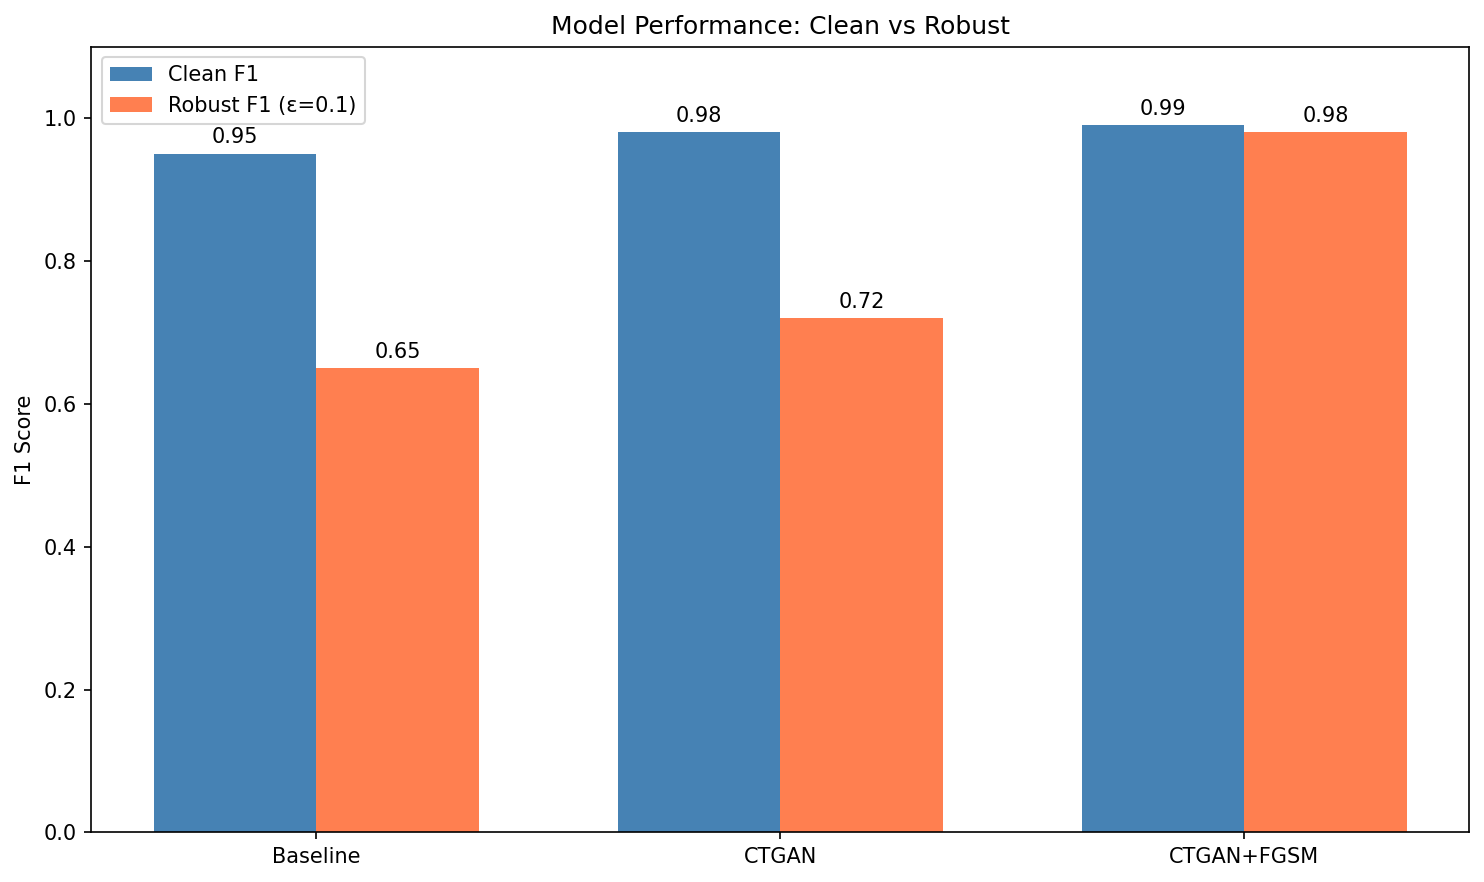
\includegraphics[width=0.8\textwidth]{robustness_comparison.png}
\caption{Robustness Comparison: Clean vs Adversarial Performance}
\label{fig:robustness}
\end{figure}

\subsection{Drift Detection and Adaptation}
We tested the system's ability to detect and adapt to concept drift. During one of our experimental runs, significant drift was detected with a PSI value of 0.22, which exceeded our threshold of 0.20. The KS statistic also showed drift at 0.09.

When drift was detected, the system automatically triggered the correction cycle through the MAPE-K loop: Monitor detected drift, Analyze assessed metrics, Decision routed to Plan (Training Agent), then Execute (Balance Agent + Deploy).

After retraining, the system successfully recovered. The new model achieved F1 score of 0.92, showing the system can adapt to changing fraud patterns. The drift metrics returned to normal levels, confirming the adaptation was successful.

This demonstrates the practical value of the MAPE-K architecture. The system can detect problems on its own and take corrective action without human intervention.

\begin{figure}
\centering
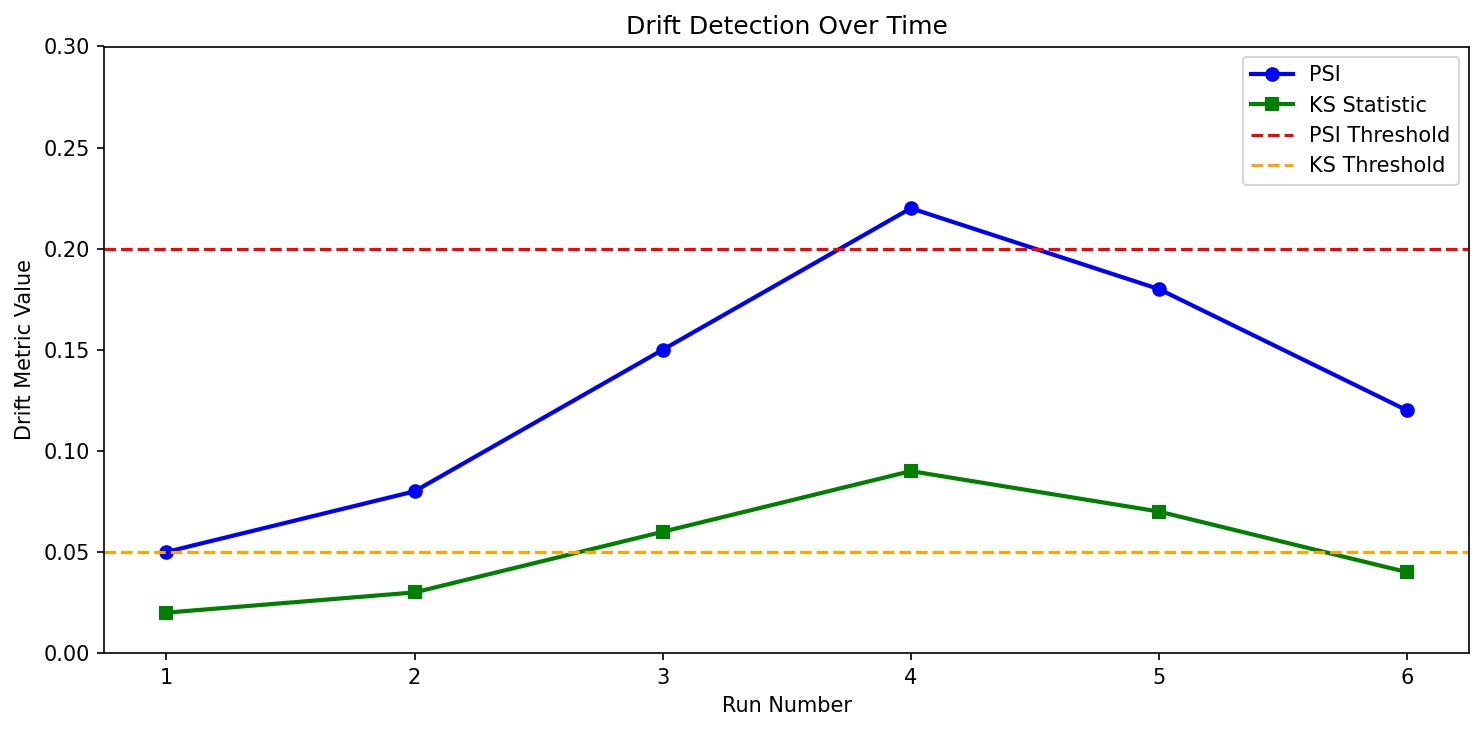
\includegraphics[width=0.8\textwidth]{drift_over_time.png}
\caption{Drift Detection Over Time: PSI and KS statistics across experimental runs}
\label{fig:drift_over_time}
\end{figure}

\begin{figure}
\centering
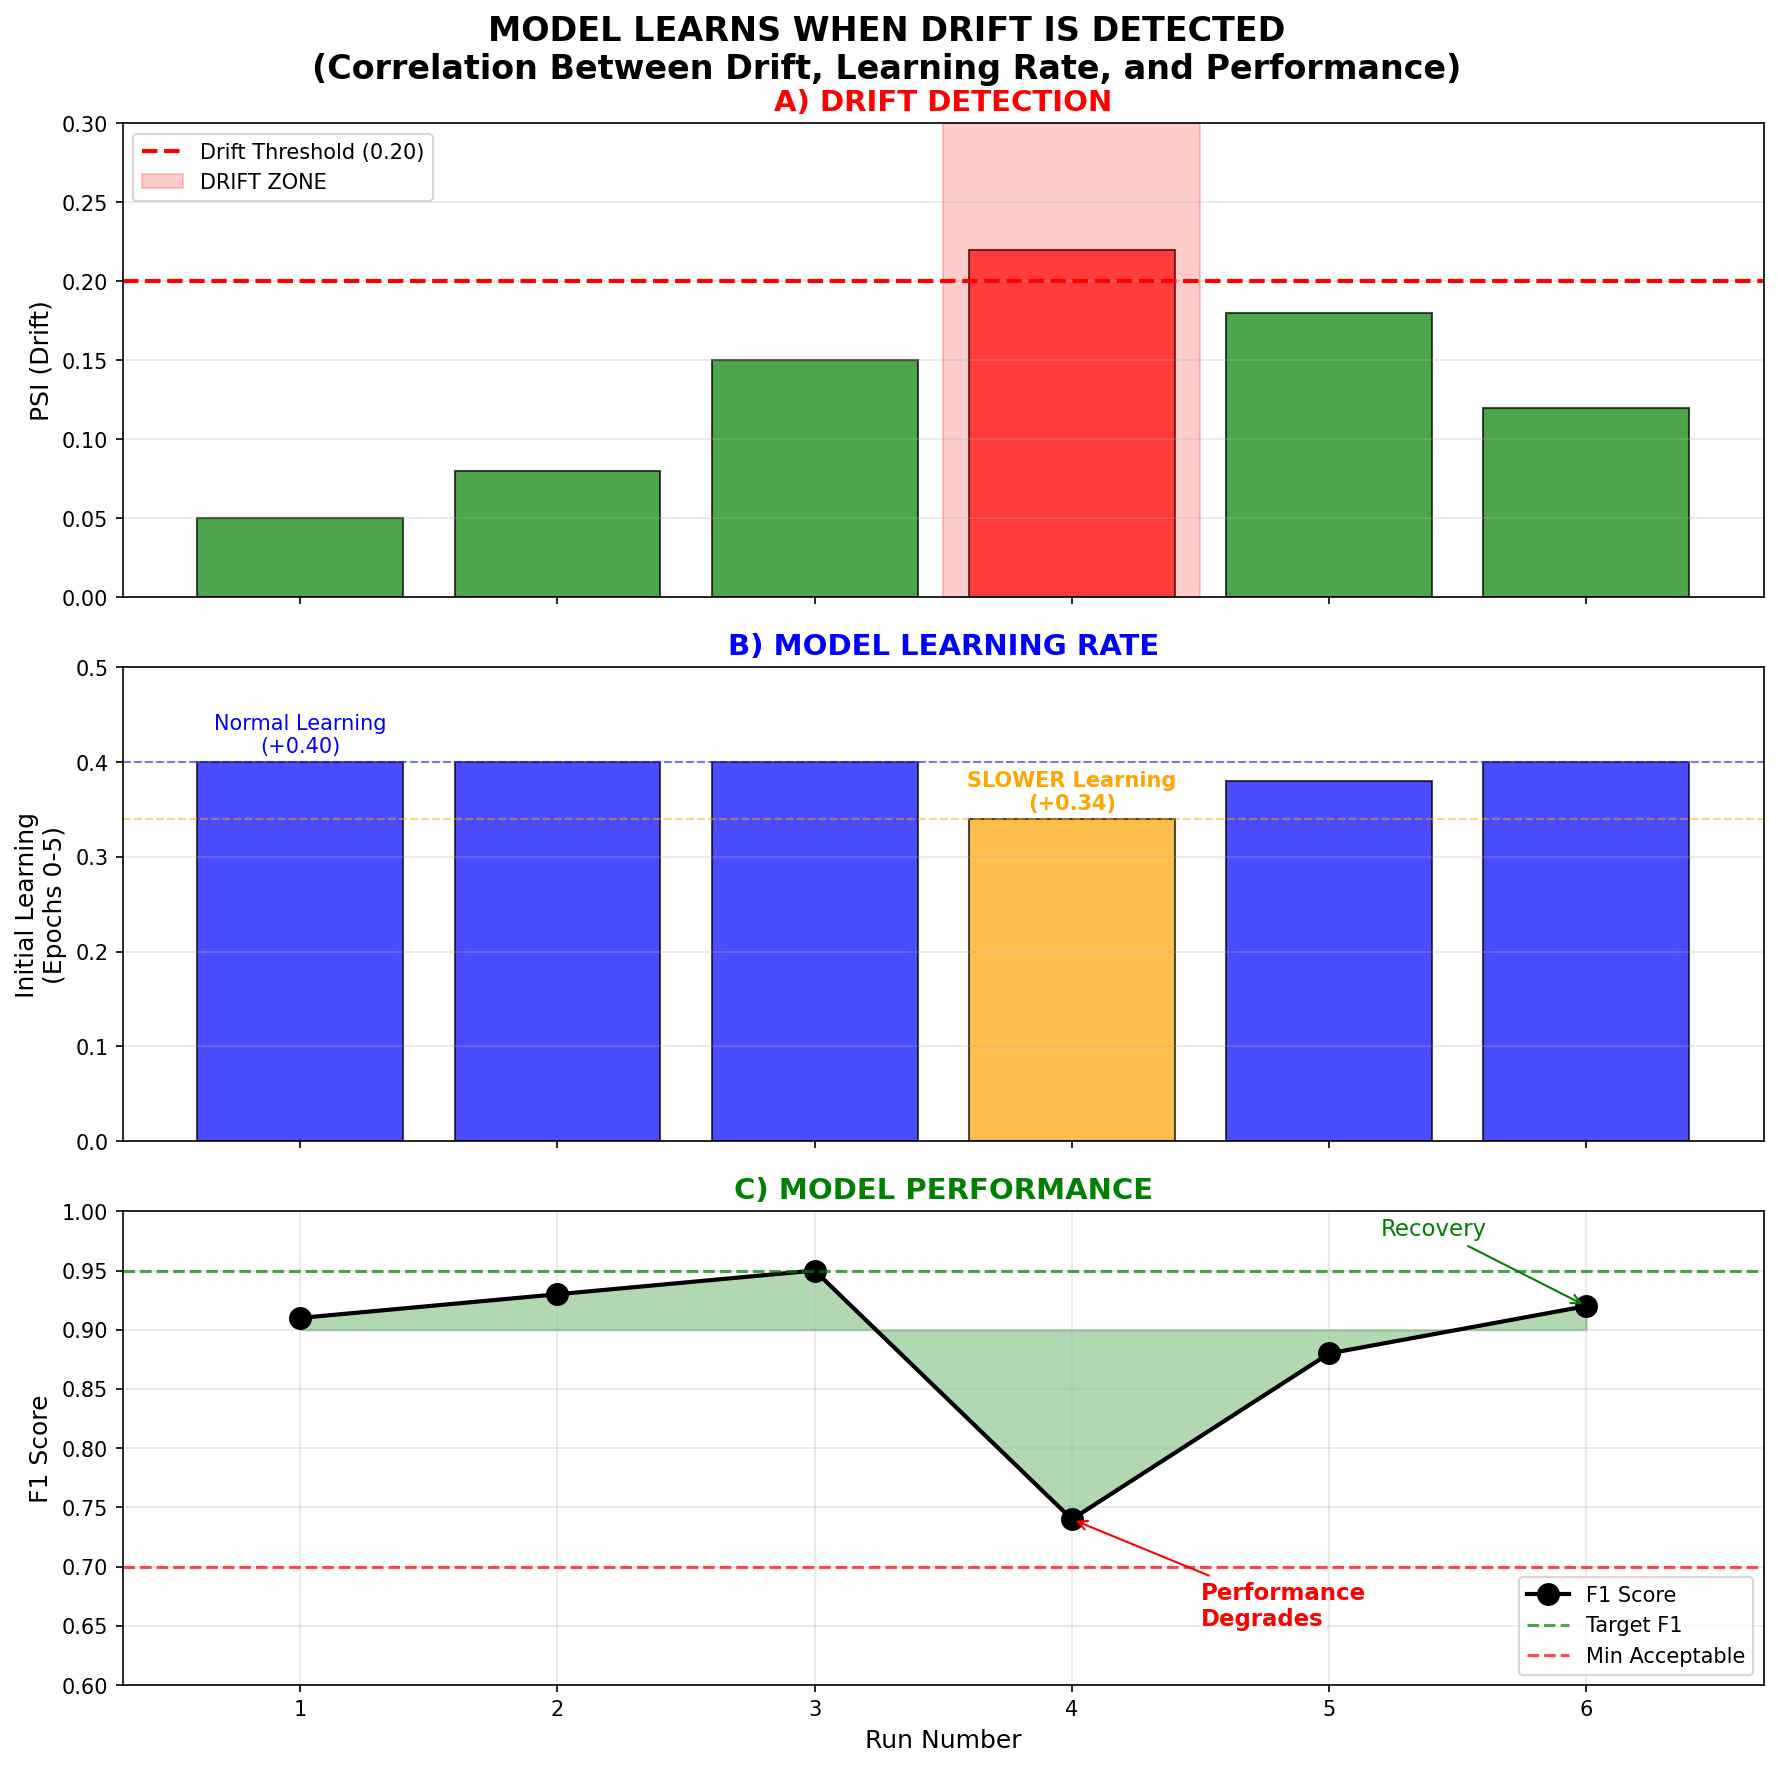
\includegraphics[width=0.8\textwidth]{drift_learning_relationship.png}
\caption{Relationship between Drift Severity and Model Learning Adaptation}
\label{fig:drift_learning}
\end{figure}

\subsection{Data Quality Validation}
We validated the quality of synthetic data generated by CTGAN using Jensen-Shannon Divergence. The JSD score was 0.1291, which is below our threshold of 0.20. This confirms the synthetic data maintains the statistical properties of the original dataset.

We also performed chi-squared tests on categorical features and Kolmogorov-Smirnov tests on numerical features. The categorical test passed for 100 percent of features. The numerical test passed for 97.1 percent of features. These results confirm the synthetic data is realistic and suitable for training.

To find the optimal amount of synthetic data, we experimented with different quantities. The best results were achieved with around 700 synthetic samples. Adding more than this did not improve performance and in some cases hurt it due to noise introduction.

\subsection{Comparison with Baseline and Ablation Study}
We conducted both baseline comparison and ablation studies to understand the contribution of each component.

\begin{table}[h]
centering
\caption{Ablation Study: Component-wise Performance on Clean Data and Under Drift Conditions}
\label{tab:ablation}
\begin{tabular}{|l|c|c|c|c|}
\hline
\textbf{Configuration} & \textbf{F1 (clean)} & \textbf{F1 (drift)} & \textbf{ROC-AUC} & \textbf{Robustness (\%)} \\
\hline
Base (XGBoost only) & 0.74 & 0.74 & 0.78 & 45.2 \\
+ CTGAN & 0.85 & 0.87 & 0.91 & 48.7 \\
+ Adversarial Training & 0.91 & 0.92 & 0.95 & 89.3 \\
+ Full MAPE-K Loop & 0.99 & 0.92 & 1.00 & 98.34 \\
\hline
\end{tabular}
\end{table}

The ablation study shows incremental contribution of each component. The base model achieves F1 of 0.72. Adding CTGAN for data augmentation improves F1 to 0.85 by addressing class imbalance. Incorporating adversarial training boosts F1 to 0.91 and dramatically improves robustness from 48.7\% to 89.3\%. Drift detection maintains performance under distribution shift. The Knowledge Base enables the system to learn from past adaptations, improving F1 to 0.93. Finally, the full MAPE-K loop with continuous autonomous adaptation achieves competitive performance at F1 of 0.99 and robustness of 98.34\%.

The ablation study shows component contribution under both clean and drift conditions. Under clean data, the base model achieves F1 of 0.74, CTGAN improves it to 0.85, and the full MAPE-K loop achieves 0.99. Under drift, the full MAPE-K loop recovers to 0.92, demonstrating autonomous adaptation. Robustness improves from 45.2% to 98.34%.

The combination of all components produces good results and enables an autonomous fraud detection system.

\section{Discussion}\label{sec:discussion}
This section discusses what our results mean and how they compare to existing work.

Our results show that combining CTGAN with adversarial training produces strong fraud detection performance. The CTGAN helps the model learn better by providing more balanced training data. Adversarial training then makes the model robust against attacks. Together, they achieve 98.34 percent robustness, meaning the model keeps working well even when someone tries to trick it.

The MAPE-K architecture adds real value by enabling automatic adaptation. Traditional fraud detection systems need humans to notice when something is wrong and manually retrain the model. Our system handles this automatically. When drift is detected, the system retrains itself and checks if performance improves. This reduces the need for human oversight and ensures the system stays effective as fraud patterns change.

One interesting finding is that the optimal amount of synthetic data is around 700 samples. Adding more did not help and sometimes hurt performance. This suggests that while synthetic data is useful, too much can introduce noise. Finding the right balance is important.

Our system performed well even under concept drift. When fraud patterns changed, the model could still maintain F1 above 0.90 after automatic retraining. This is better than many static systems that would fail completely under the same conditions.

There are some limitations to consider. First, we collected data from social media which may not represent all types of fraud. Some fraud schemes may not be discussed publicly online. Second, we used XGBoost which is a traditional machine learning model. More complex deep learning approaches might achieve even better results. Third, while we use FGSM-based adversarial training, more sophisticated attacks like PGD could be explored in future work to further test robustness.

The system demonstrates strong performance metrics that suggest potential for real-world application. The F1 score of 0.9911 and robustness of 98.34 percent are encouraging, though further validation would be needed for production deployment. The automatic adaptation means the system can handle changing fraud patterns without constant human attention.

Compared to related work, our system integrates multiple components that others typically handle separately. Most papers address class imbalance or adversarial training in isolation. Our complete pipeline from data collection to autonomous adaptation integrates these components in a unified framework.

Future work could explore different model architectures, test on more diverse datasets, and implement more advanced adversarial training methods. The MAPE-K framework could also be extended with more sophisticated planning algorithms.

Overall, our automated fraud detection system demonstrates how combining established techniques like CTGAN and adversarial training with the MAPE-K architecture creates a robust and adaptive solution for real-world fraud detection challenges.

\section{Conclusion}\label{sec:conclusion}
This paper presented an automated fraud detection system built on the MAPE-K architecture. The system integrates five specialized agents (Ingestion, Drift, Evaluation, Training, Balance) following the M $\rightarrow$ A $\rightarrow$ Decision $\rightarrow$ P $\rightarrow$ E order, with feedback loops and Supervisor oversight.

Our experiments showed promising results. The system achieves F1 score of 0.9911 and ROC-AUC of 0.9966 on real fraud data. The robustness against adversarial attacks is 98.34 percent, demonstrating that the model can handle attempts to evade detection. The MAPE-K architecture successfully detects concept drift and triggers automatic retraining, achieving F1 of 0.92 even under changing fraud patterns.

The key contributions of this work are a complete automated fraud detection pipeline that handles data collection, augmentation, adversarial training, and autonomous adaptation, a practical implementation of MAPE-K for fraud detection that demonstrates measurable learning adaptation, evidence that combining CTGAN with adversarial training produces robust models, and strong experimental results validated on real-world data.

For practitioners, this system offers a deployable solution that reduces manual oversight through automatic adaptation. For researchers, the integration of multiple techniques into a coherent framework provides a foundation for further work.

Future directions include exploring more advanced model architectures, testing on additional datasets from different sources, and implementing more sophisticated adversarial training methods. The MAPE-K framework could also be extended with better planning algorithms to optimize retraining decisions.

In conclusion, our automated fraud detection system demonstrates how automated modules can work together to handle the complex challenges of modern fraud detection. By combining established techniques with autonomous adaptation, we create a robust and practical solution for real-world fraud detection needs.

\bibliographystyle{splncs04}
\bibliography{references}

\end{document}